\documentclass[journal,12pt,twocolumn]{IEEEtran}
\usepackage{graphicx}
\graphicspath{{./figs/}}{}
\usepackage{amsmath,amssymb,amsfonts,amsthm}
\newcommand{\myvec}[1]{\ensuremath{\begin{pmatrix}#1\end{pmatrix}}}
\usepackage{listings}
\usepackage{watermark}
\usepackage{titlesec}
\let\vec\mathbf

\titlespacing{\subsection}{0pt}{\parskip}{-3pt}
\titlespacing{\subsubsection}{0pt}{\parskip}{-\parskip}
\titlespacing{\paragraph}{0pt}{\parskip}{\parskip}
\newcommand{\figuremacro}[5]{
    
}
\lstset{
frame=single, 
breaklines=true,
columns=fullflexible
}
\thiswatermark{\centering \put(0,-105.0){
\includegraphics[scale=0.05]{iitlogo.jpg}} }

\sloppy
\title{\mytitle}
\title{
Conic Assignment 
}
\author{T.Siva Parvathi(FWC22089)}
\begin{document}
\maketitle
\tableofcontents
\bigskip


\section{\textbf{problem}}
Q.The locus of the mid-point of the lines segment joining the focus to a moving point on the parabola $y^2$=4a$x$ is another parabola with directrix

\section{\textbf{solution}}
The standard conic equation is,\\
\begin{align}
\label{eq:one}
\vec{x}^\top\vec{Vx}+2\vec{u}^\top\vec{x}+f=0
\end{align} 
 where,\\
$\vec{V}=\myvec{0&0 \\0&1}$\\ $\vec{u}=\myvec{-2a\\0}$ and $f=0$ \\
let moving point on the parabola be 'q',then the equation is,
\begin{align}
\label{eq:two}
\vec{q}^\top\vec{Vq}+2\vec{u}^\top\vec{q}+f=0
\end{align}
the mid-point when line segment joining the focus to moving point on the parabola be 'h'.
\begin{align}
\label{eq:three}
\vec{h}=\frac{\vec{q+F}}{2}
\end{align}
\begin{align}
\label{eq:four}
\vec{q}=2\vec{h}-\vec{F}
\end{align}
Substitute \eqref{eq:four} in \eqref{eq:two}\\
\begin{align}
\label{eq:five}
(2\vec{h}-\vec{F})^\top\vec{V}(2\vec{h}-\vec{F})+2\vec{u}^\top(2\vec{h}-\vec{F})+f=0
\end{align}
By solving we get the locus parabola equation is, \\
\begin{align}
\label{eq:six}
\vec{x}^\top\vec{V}_{1}\vec{x}+2\vec{u}_{1}^\top\vec{x}+f_1=0
\end{align} 
where,\\
$\vec{V}_{1}=\myvec{0&0 \\0&1}$\\ $\vec{u}_{1}=\myvec{-a\\0}$ and $f_1=a^2$ \\
The new parabola equation in terms of old parabola equation is,\\
\begin{center}
$\vec{x}^\top\vec{V}\vec{x}+\vec{u}^\top\vec{x}+(f+d)=0$
\end{center}
The directrix of a conic is given by,
\begin{align}
\label{eq:seven}
\vec{n}^\top\vec{x}=c
\end{align}
The directrices of \eqref{eq:six} is given by,\\
\begin{align}
\vec{n}=\sqrt{\lambda_2}\vec{p}_{1}\\
c=\frac{\|\vec{u}\|^2-\lambda_2 f}{2\vec{u}^\top\vec{n}} , e=1
\end{align}
where the eigen values and eigen vectors are,\\
\begin{align}
\label{eq:eight}
\lambda_1=0 , \lambda_2=1\\
\vec{p}_{1}=\myvec{1\\0}, \vec{p}_{2}=\myvec{0\\1} 
\end{align}
substituting values in \eqref{eq:eight} we get,\\
\begin{align}
\label{eq:nine}
\vec{n}=\myvec{1\\0}
\end{align}
substituting values in \eqref{eq:nine},\\
$c=\frac{a^2-a^2}{2\myvec{-a & 0}\myvec{1\\0}}$\\
\begin{align}
\label{eq:ten}
c=0
\end{align}
put n and c in directrix equation we get,
\begin{align}
\label{eq:eleven}
\myvec{1&0}\vec{x}=0
\end{align}
        Therefore,the locus of the mid-point of the lines segment joining the focus to a moving point on the parabola $y^2$-$4ax=0$ is another parabola $y^2$-$2ax$+$a^2=0$ with directrix $x=0$.\\

\section{\textbf{figure}}
\begin{figure}[h]
    \centering
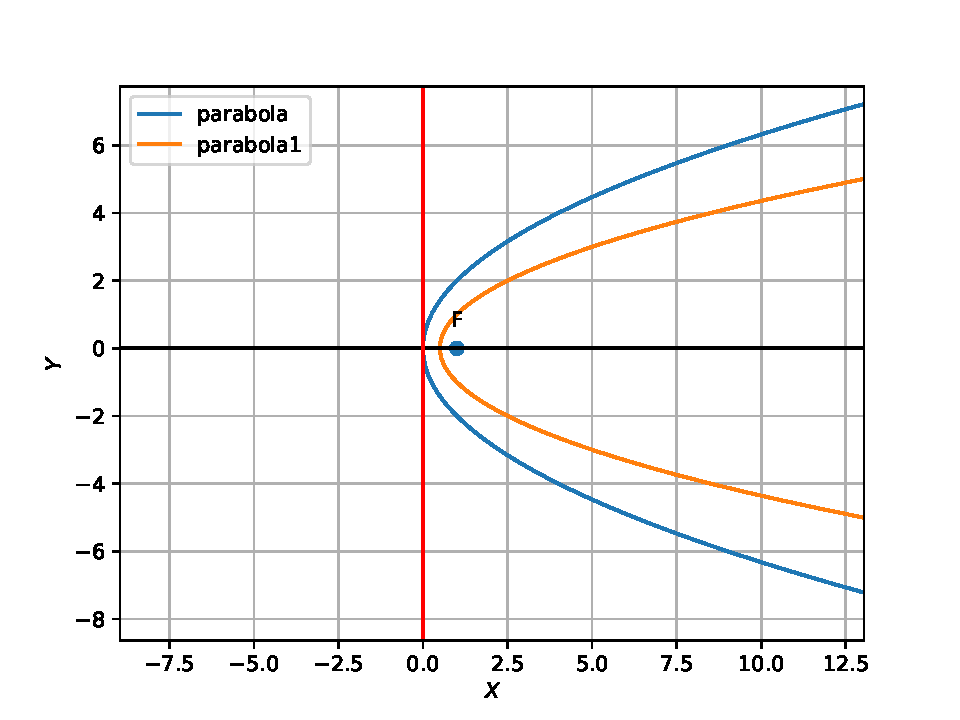
\includegraphics[width=\columnwidth]{cofig.pdf}
\caption{labeling}
    \label{fig:my_label}
\end{figure}

\section{\textbf{software}}
\begin{lstlisting}
https://github.com/sivaparvathi-tungala/fwc_module_1/tree/main/conic
\end{lstlisting}
\end{document}